\section*{Лекция 4. Продолжение градиентного спуска. Введение в классификацию}
\subsection*{Изменение вида градиентного шага}

Градиентный спуск можно улучшить 2 основными способами. Например, с помощью \textbf{momentum}, или «инерции». Идея в том, чтобы учитывать прошлые градиенты и накапливать скорость в направлении движения. Если долго идти в одном направлении, momentum усиливает шаг, помогая пройти через небольшие препятствия (минимумы, которые не являются оптимальными). 

Рассмотрим следующее изображение:
\begin{figure}[H]
    \centering
    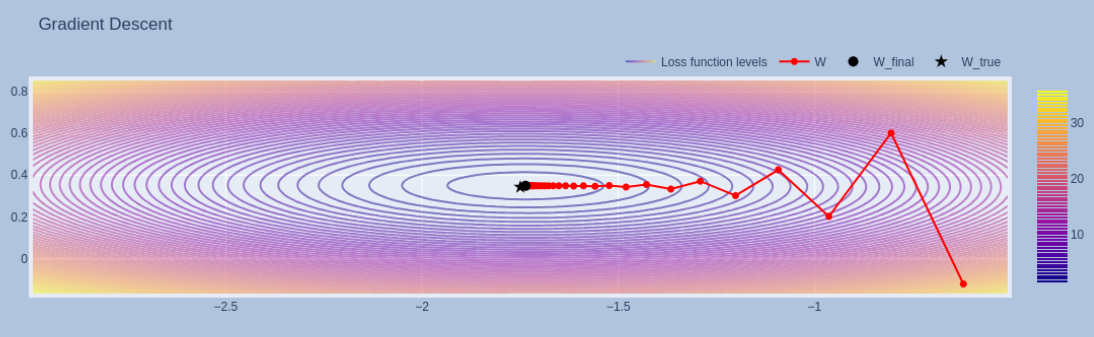
\includegraphics[width=0.9\linewidth]{media/fbgd_trajectory.png}
\end{figure}

На нём мы видим, что по горизонтальной оси --- всё хорошо, градиент постепенно шагает в оптимум (на рисунке "--- в самом центре линий уровня). Однако по вертикальной оси наблюдаются т.н. осцилляции --- это когда значение бегает то вверх, то вниз.

Заметим, что если мы просто проссумируем эти векторы, то мы исправим эту проблему и, соответственно, алгоритм будет подбирать значения весов гораздо быстрее.

Формально шаг с momentum вычисляется через вспомогательный вектор $v_t$, который обновляется как комбинация предыдущего шага и текущего градиента:
\[
v_t = \gamma v_{t-1} + \eta \nabla J(w_t),
\]
а параметры обновляются по формуле
\[
w_{t+1} = w_t - v_t.
\]
Здесь $\gamma$ — коэффициент «памяти», обычно около 0.9. Чем больше $\gamma$, тем больше мы хотим учитывать значение предыдущего градиента. 

\newpage
\subsection*{Градиентный спуск на разреженных данных}

Следующая проблема касается только \texttt{SGD} и \texttt{mini batch GD}.

Разреженные данные "--- данные, в которых определённый признак очень часто принимает нулевое значение. И это далеко не редкая проблема --- вспомните метод \texttt{One Hot Encoding}, который представляет категориальные признаки как бинарный вектор.

Нас это беспокоит потому, что при обновлении весов на этих самых нулевых объектах вес не будет изменяться (т.к. частная производная будет равна 0). Значит, скорее всего мы хотим, чтобы на этих объектах был какой"=то свой, независимый \texttt{learing rate}, который будет жить своей жизнью.

Давайте посмотрим на одно из решений этой проблемы "--- \texttt{AdaGrad}:
\[
G_{kj} = G_{k-1, j} + (\nabla_w Q(w^{(k-1)}))_j^2
\]

\[
w_j^{(k)} = w_j^{(k-1)} - \frac{\eta_k}{\sqrt{G_{kj} + \epsilon}}(\nabla_w Q(w^{(k-1)}))_j
\]
$(k, j)$ "--- номер итерации, номер параметра.

Тут уже заметно сложнее. Итак, в матрице $G$ на позиции $kj$ мы храним, насколько много мы уже обучали $w_j$. Накапливаем квадрат градиента, чтобы сильнее подчеркнуть контраст: веса, которые уже сильно изменились, надо изменять поменьше, а те веса, которые изменились мало, надо изменять сильнее.

В зависимости от этого, мы изменяем значение \texttt{learning rate} (тут под шагом подразумевается вся дробь целиком во втором уравнении). Если объект с ненулевым значением признака попадается впервые, то тогда $G_{kj} = 0$ и градиент шагает <<со свежей головой>>. 

Тут важно понять, что по факту $G$ есть диагональная матрица (т.е. элементы есть только на диагонали, всё остальное "--- 0). На первом таком элементе диагонали мы храним, сколько мы шагали для первого объекта выборки, на втором --- по второму объекту и т.д.

\newpage
Проблема: $G_{kj}$ только увеличивается, и замедление шага может оказаться слишком быстрым. Для этого мы воспользуемся модификацией "--- \texttt{RMSProp}. Отличие лишь в том, что $G_{kj}$ мы теперь вычисляем с некоторым затуханием:
\[
G_{kj} = \alpha G_{k-1, j} + (1 - \alpha)(\nabla_w Q(w^{(k-1)}))_j^2
\]
Кстати, этот метод придумал Джеффри Хинтон "--- великий человек в области глубокого обучения.
Но интереснее, как он его придумал "--- объясняя на своих занятиях \texttt{AdaGrad}, он просто между строк вкинул, что <<можно вот такие вот коэффициенты добавить и будет лучше>>.